\subsection{I-Regler} % (fold)
\label{sub:I-Regler}
\begin{frame}
    \frametitle{I-Regler}
    \framesubtitle{}
    \begin{block}{Versuchsziel}
        \begin{itemize}
            \item Untersuchung der I-Regelung 
            \item Untersuchung des "anti-wind-ups"
        \end{itemize}
    \end{block}
\end{frame}
\begin{frame}
    \frametitle{I-Regler}
    \framesubtitle{}
    \begin{columns}[c]
        \column{0.5\textwidth}
             \begin{block}{}
                \begin{itemize} 
                    \item Durch fit am Graphen
                        \begin{itemize}
                            \item $|\Delta T| \leq 1K$ bei $t=361s$
                            \item $|\Delta T| \leq 0.1K$ bei $t=651s$
                        \end{itemize}
                \end{itemize}
             \end{block}
        \column{0.5\textwidth}
            \begin{figure}[H]
            \begin{center}
                    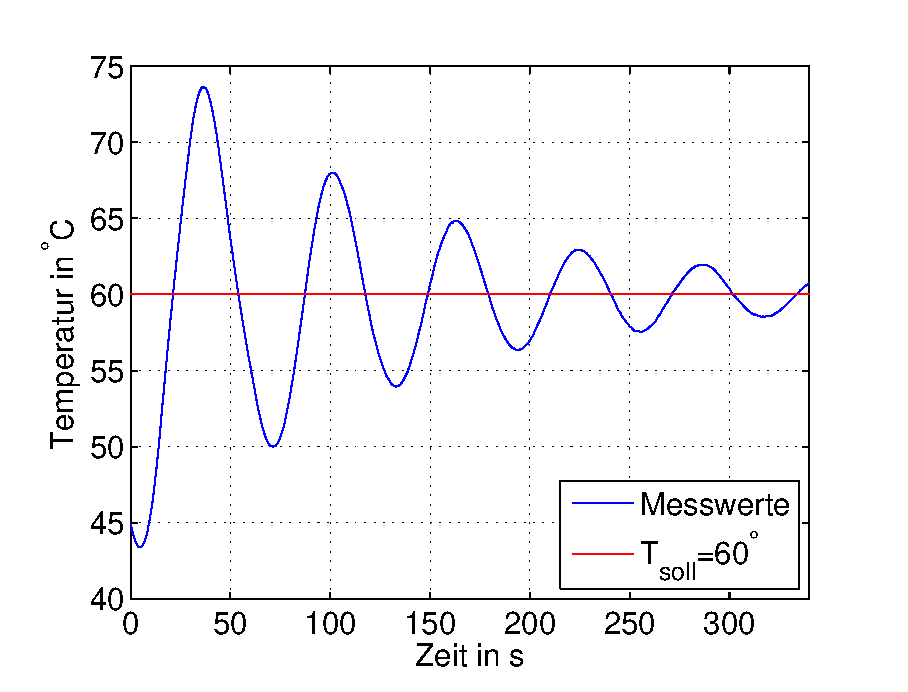
\includegraphics[scale=0.3]{./img/plots/2_c_100.eps}
            \end{center}
            \end{figure}
            \begin{figure}[H]
            \begin{center}
                    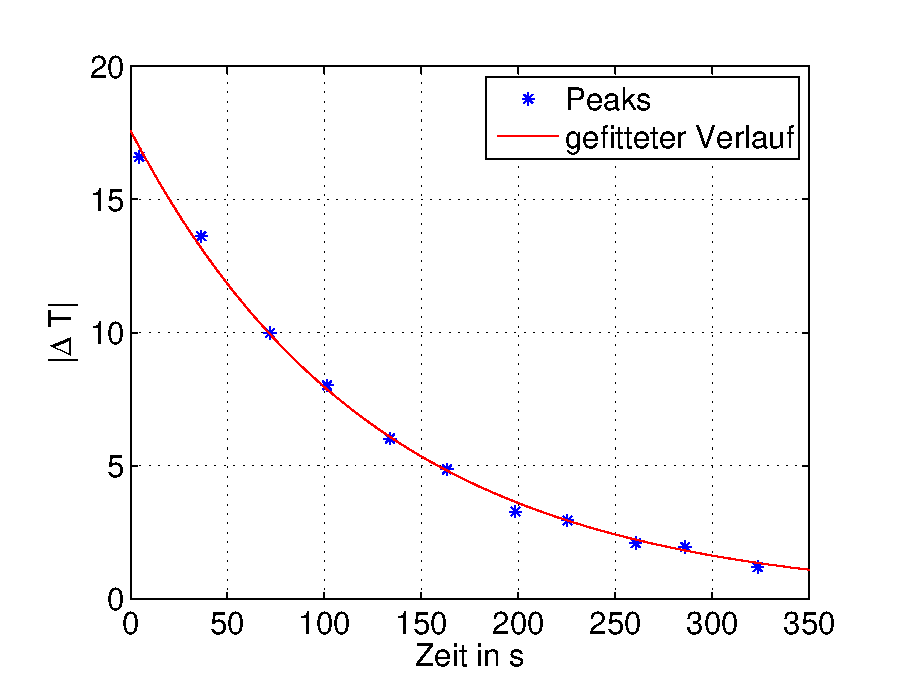
\includegraphics[scale=0.3]{./img/plots/2_c_100_Peaks.eps}
            \end{center}
            \end{figure}
     \end{columns}
\end{frame}
\begin{frame}
    \frametitle{anti-Windup}
    \framesubtitle{}
    \begin{columns}[c]
        \column{0.5\textwidth}
            \begin{block}{anti-windup}
                \begin{itemize}
                    \item AW-Funktion limitiert Werte so dass
                        \begin{itemize}
                            \item $P+I+D = I_{max}$ 
                            \item $P+I+D = 0$ 
                        \end{itemize}
                        wenn sonst $I_{max}$ übeschritten würde
                \end{itemize}
            \end{block}    
            \begin{block}{}
                \begin{itemize}
                    \item Kurve läuft schneller gegen geringere Amplitutde
                    %\item
                    %\begin{tabular}{c|c|}
                    %    & T(1K) & T(0.1K) \\
                    %    ohne AWU:& 361.2& 651.2 \\
                    %    mit AWU:& 327.1& 615.1 
                    %\end{tabular}
                \end{itemize}
            \end{block}
        \column{0.5\textwidth}
            \begin{figure}[H]
            \begin{center}
                    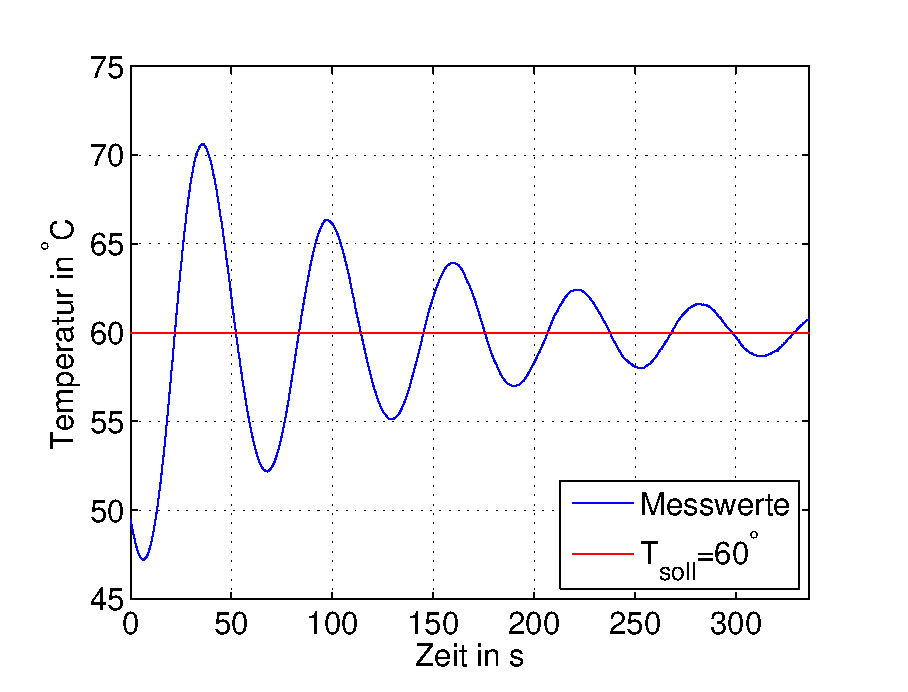
\includegraphics[scale=0.3]{./img/plots/2_c_100_wind.eps}
            \end{center}
            \end{figure}
            \begin{figure}[H]
            \begin{center}
                    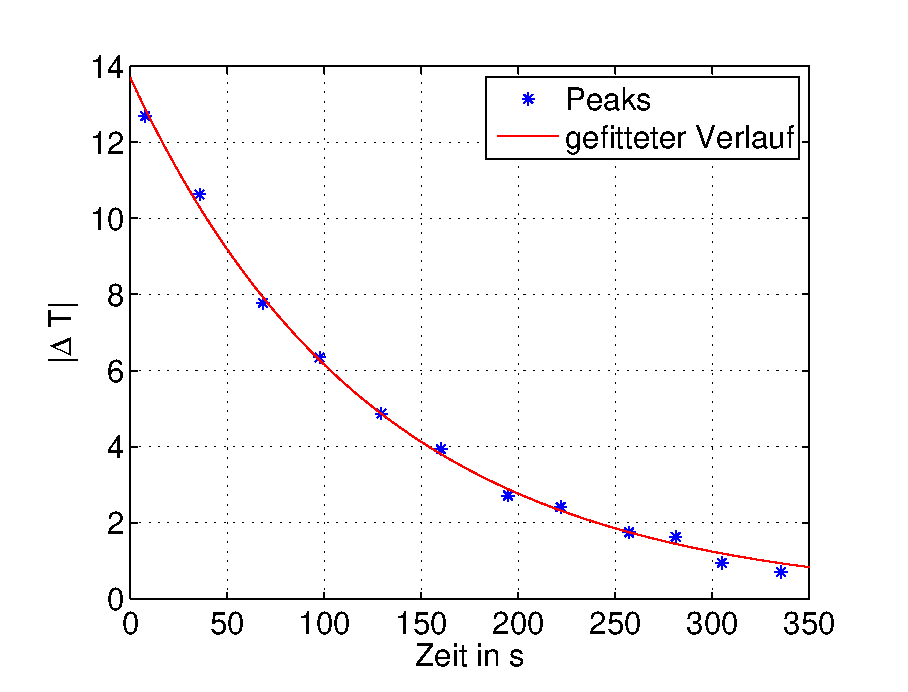
\includegraphics[scale=0.3]{./img/plots/2_c_100_Peaks_wind.eps}
            \end{center}
            \end{figure}
    \end{columns}
\end{frame}
% subsection I-Regler (end)
